Der allgemeine Ablauf der Anwendung kann in der Abbildung~\ref{fig:ProximetyUIFlow} entnommen werden. Anschliessend folgen alle bisher definierten Fenster der Variante 1.

\def\guivarone{bilder/guivariante1/}
\FloatBarrier
\begin{figure}[hp]
	\centering
	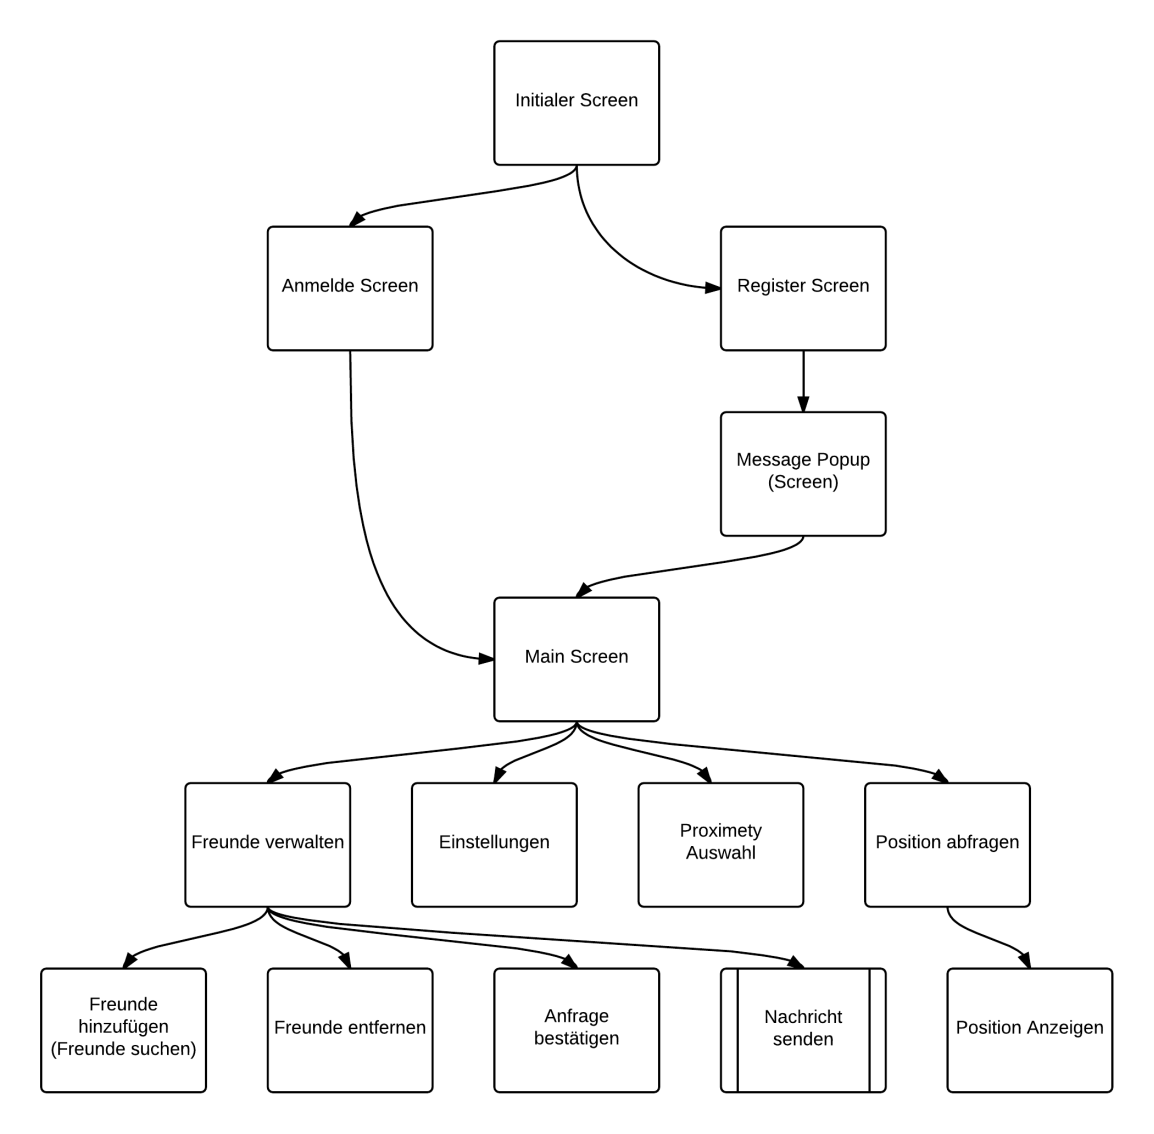
\includegraphics[scale=0.4]{ProximetyUIFlow.png}
	\caption{Design Flow Diagramm}
	\label{fig:ProximetyUIFlow}
\end{figure}
\FloatBarrier
\begin{figure}[H]
	\centering
	\begin{subfigure}[h]{0.3\textwidth}
		\includegraphics[width=1\textwidth]{\guivarone{initialer_screen.png}}
		\caption{Initiales Fenster}
		\label{fig:initscreenone}
	\end{subfigure}%
	\qquad %add desired spacing between images, e. g. ~, \quad, \qquad, \hfill etc.
	%(or a blank line to force the subfigure onto a new line)
	\begin{subfigure}[h]{0.3\textwidth}
		\includegraphics[width=1\textwidth]{\guivarone{register_screen.png}}
		\caption{Registrierungsfenster}
		\label{fig:registerscreenone}
	\end{subfigure}
	\caption{Initialer und Registrierungsfenster}
\end{figure}
\begin{figure}[H]
	\centering
	\begin{subfigure}[h]{0.3\textwidth}
		\includegraphics[width=1\textwidth]{\guivarone{messages_popup_screen.png}}
		\caption{Benachrichtigungsfenster}
		\label{fig:popmesagesscreenone}
	\end{subfigure}%
	\qquad %add desired spacing between images, e. g. ~, \quad, \qquad, \hfill etc.
	%(or a blank line to force the subfigure onto a new line)
	\begin{subfigure}[h]{0.3\textwidth}
		\includegraphics[width=1\textwidth]{\guivarone{main_screen.png}}
		\caption{Hauptfenster}
		\label{fig:mainscreenone}
	\end{subfigure}
	\caption{Benachrichtigungs- und Hauptfenster}
\end{figure}
\begin{figure}[H]
	\centering
	\begin{subfigure}[h]{0.3\textwidth}
		\includegraphics[width=1\textwidth]{\guivarone{freunde_verwalten.png}}
		\caption{Freunde Verwaltungsfenster}
		\label{fig:friendmgmtscreenone}
	\end{subfigure}%
	\qquad %add desired spacing between images, e. g. ~, \quad, \qquad, \hfill etc.
	%(or a blank line to force the subfigure onto a new line)
	\begin{subfigure}[h]{0.3\textwidth}
		\includegraphics[width=1\textwidth]{\guivarone{freunde_hinzufgen_freunde_suchen.png}}
		\caption{Freunde hinzufügen (Freunde suchen)}
		\label{fig:friendaddsearchscreenone}
	\end{subfigure}
	\caption{Freunde Verwaltungs- und Hinzufügefenster (Freunde suchen) }
\end{figure}
\begin{figure}[H]
	\centering
	\begin{subfigure}[h]{0.3\textwidth}
		\includegraphics[width=1\textwidth]{\guivarone{freunde_hinzufgen_offene_anfragen.png}}
		\caption{Freunde hinzufügen (Offene Anfragen)}
		\label{fig:friendaddrequestscreenone}
	\end{subfigure}%
	\qquad %add desired spacing between images, e. g. ~, \quad, \qquad, \hfill etc.
	%(or a blank line to force the subfigure onto a new line)
	\begin{subfigure}[h]{0.3\textwidth}
		\includegraphics[width=1\textwidth]{\guivarone{freunde_entfernen.png}}
		\caption{Freunde entfernen}
		\label{fig:friendremovescreenone}
	\end{subfigure}
	\caption{Freunde Entfernen- und Hinzufügefenster (Offene Anfragen) }
\end{figure}
\begin{figure}[H]
	\centering
	\begin{subfigure}[h]{0.3\textwidth}
		\includegraphics[width=1\textwidth]{\guivarone{proximety_auswahl.png}}
		\caption{Proximety Auswahl}
		\label{fig:proxchoicescreenone}
	\end{subfigure}%
	\qquad %add desired spacing between images, e. g. ~, \quad, \qquad, \hfill etc.
	%(or a blank line to force the subfigure onto a new line)
	\begin{subfigure}[h]{0.3\textwidth}
		\includegraphics[width=1\textwidth]{\guivarone{position_abfragen_auswahl.png}}
		\caption{Position abfragen Auswahl}
		\label{fig:posrequestchoicescreenone}
	\end{subfigure}
	\caption{Proximety Auswahl- und Position Abfragefenster }
\end{figure}
\begin{figure}[H]
	\centering
	\begin{subfigure}[h]{0.3\textwidth}
		\includegraphics[width=1\textwidth]{\guivarone{anfrage_besttigen.png}}
		\caption{Anfrage bestätigen}
		\label{fig:requestconfirmscreenone}
	\end{subfigure}%
	\qquad %add desired spacing between images, e. g. ~, \quad, \qquad, \hfill etc.
	%(or a blank line to force the subfigure onto a new line)
	\begin{subfigure}[h]{0.3\textwidth}
		\includegraphics[width=1\textwidth]{\guivarone{anmelde_screen.png}}
		\caption{Anmeldefenster}
		\label{fig:loginscreenone}
	\end{subfigure}
	\caption{Anfrage Bestätigungs- und Anmeldefenster }
\end{figure}
\begin{figure}[H]
	\centering
	\begin{subfigure}[h]{0.3\textwidth}
		\includegraphics[width=1\textwidth]{\guivarone{position_anzeigen.png}}
		\caption{Position anzeigen}
		\label{fig:displayposscreenone}
	\end{subfigure}%
	\qquad %add desired spacing between images, e. g. ~, \quad, \qquad, \hfill etc.
	%(or a blank line to force the subfigure onto a new line)
	\begin{subfigure}[h]{0.3\textwidth}
		\includegraphics[width=1\textwidth]{\guivarone{proximety_alarm.png}}
		\caption{Proximety Alarm}
		\label{fig:proxalertscreenone}
	\end{subfigure}
	\caption{Positions- und Proximety Alarm Anzeigefenster}
\end{figure}
\begin{figure}[H]
	\centering
	\begin{subfigure}[h]{0.3\textwidth}
		\includegraphics[width=1\textwidth]{\guivarone{freund_details.png}}
		\caption{Details Freunde}
		\label{fig:detailfriendsscreenone}
	\end{subfigure}%
	\qquad %add desired spacing between images, e. g. ~, \quad, \qquad, \hfill etc.
	%(or a blank line to force the subfigure onto a new line)
	\begin{subfigure}[h]{0.3\textwidth}
		\includegraphics[width=1\textwidth]{\guivarone{einstellungen.png}}
		\caption{Einstellungen}
		\label{fig:settingsscreenone}
	\end{subfigure}
	\caption{Freunde Detail- und Einstellungsfenster}
\end{figure}
